% Metrics report for the organisers' "Scoring weights" slide.
% Official metrics: `vineyard eval-examples --gates` on the organisers' 2 example tiles.
% Survey numbers: run rc10f, route from post run 20260927T1400-post-rc10f-pretest (organizers' pre-test START)
% (root measurements.csv, route.geojson, targets.geojson).
\documentclass[10pt,a4paper]{article}
\usepackage[margin=16mm,top=14mm,bottom=16mm]{geometry}
\usepackage[T1]{fontenc}
\usepackage[utf8]{inputenc}
\usepackage{helvet}
\renewcommand{\familydefault}{\sfdefault}
\usepackage{booktabs,tabularx,array,xcolor,tikz,enumitem}
\usepackage[hidelinks]{hyperref}

\definecolor{night}{HTML}{1B2B25}
\definecolor{muted}{HTML}{5F6B66}
\definecolor{cCan}{HTML}{79AC61}
\definecolor{cWas}{HTML}{ECA95E}
\definecolor{cAxe}{HTML}{55B0AF}
\definecolor{cMea}{HTML}{93BCB1}
\definecolor{cRou}{HTML}{EB7866}
\definecolor{cEng}{HTML}{A497E8}

\setlength{\parindent}{0pt}
\setlength{\parskip}{3pt}
\setlist{nosep,leftmargin=12pt}
\newcolumntype{Y}{>{\raggedright\arraybackslash}X}

\newcommand{\crit}[3]{%
  \par\vspace{7pt}%
  {\color{#1}\rule[-2pt]{6pt}{12pt}}\hspace{5pt}{\large\bfseries\color{night}#2}\hfill{\bfseries\color{#1}#3}\par
  \vspace{-2pt}{\color{#1}\rule{\linewidth}{0.8pt}}\par\vspace{2pt}}
\newcommand{\kpi}[2]{\begin{tabular}[t]{@{}l@{}}{\Large\bfseries\color{night}#1}\\[-1pt]{\scriptsize\color{muted}#2}\end{tabular}}

\begin{document}
\color{night}

{\LARGE\bfseries Sireț3 Vineyard AI Field Challenge — metrics report}\par
\vspace{2pt}
{\large Team Solemtrix \textperiodcentered{} GigaHack 2026 \textperiodcentered{} 27 September 2026, 14:00}\par
\vspace{4pt}
{\small\color{muted}Numbers are grouped by the six criteria of the organisers' ``Scoring weights'' slide.
\textbf{Official metrics} are computed with the challenge metric definitions on the organisers' 2 reference
tiles (\texttt{vineyard eval-examples --gates}). \textbf{Survey numbers} cover all 311 tiles (81.5\,ha)
and come from the published deliverables in the repository root: \texttt{measurements.csv},
\texttt{route.geojson}, \texttt{targets.geojson} (annotation run \texttt{rc10f}, route run
\texttt{20260927T1400-post-rc10f-pretest}, route from the organizers' pre-test START). All geometry is EPSG:32635, measured planar.}\par

\vspace{6pt}
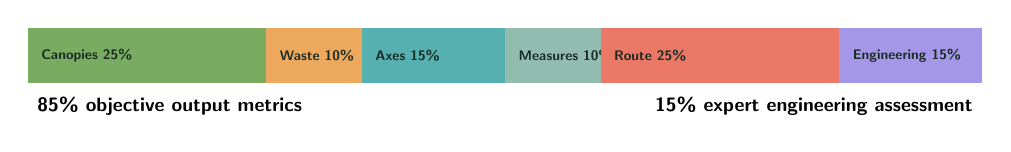
\begin{tikzpicture}[x=\linewidth/100,y=1mm]
  \foreach \s/\w/\c/\t in {0/25/cCan/Canopies 25\%, 25/10/cWas/Waste 10\%, 35/15/cAxe/Axes 15\%,
                           50/10/cMea/Measures 10\%, 60/25/cRou/Route 25\%, 85/15/cEng/Engineering 15\%}{
    \fill[\c] (\s,0) rectangle ++(\w,7);
    \node[anchor=west,font=\tiny\bfseries,text=night] at (\s+0.4,3.5) {\t};
  }
  \node[anchor=north west,font=\scriptsize\bfseries] at (0,-0.5) {85\% objective output metrics};
  \node[anchor=north east,font=\scriptsize\bfseries] at (100,-0.5) {15\% expert engineering assessment};
\end{tikzpicture}

% ------------------------------------------------------------------ summary
\vspace{4pt}
{\large\bfseries At a glance}\par\vspace{2pt}
{\small
\begin{tabularx}{\linewidth}{@{}l r Y@{}}
  \toprule
  \textbf{Criterion} & \textbf{Weight} & \textbf{Headline result} \\
  \midrule
  Canopies    & 25\% & official canopy score \textbf{0.876} (IoU 0.856, F1 0.905); inter-row IoU 0.960; 13,702 plants on the survey \\
  Waste       & 10\% & 1,331 candidates $\rightarrow$ CLIP probe $\rightarrow$ SAM\,3 $\rightarrow$ team approval: \textbf{11} boxes exported, 0 unreviewed \\
  Axes        & 15\% & row F1 \textbf{1.00} (51/51), grouping F1 1.00, attributes 1.00; 674 rows in 44 blocks on the survey \\
  Measures    & 10\% & official counts score \textbf{0.973}; row-length error 0.05\%, canopy-area error 1.4\% (0.3\% pooled) \\
  Route       & 25\% & \textbf{24.18\,km} closed route from the pre-test START, 795 targets visited, 1.29\% outside (limit 2\%), 65\% shorter than the baseline tour \\
  Engineering & 15\% & tiles $\rightarrow$ deliverables in $\approx$20\,min on a laptop; 2,378 tests, CI, export validator (311 tiles, 0 errors) \\
  \bottomrule
\end{tabularx}}

% ------------------------------------------------------------------ canopies
\crit{cCan}{Canopies}{25\%}
\kpi{0.876}{canopy score (official)}\hfill
\kpi{0.856}{canopy IoU}\hfill
\kpi{0.905}{canopy F1 (0.945 on r006\_c004)}\hfill
\kpi{0.960}{inter-row IoU}\hfill
\kpi{585/650}{reference plants matched}
\par\vspace{3pt}
{\small
\begin{itemize}
  \item \textbf{Method:} Lab a* vegetation threshold restricted to each row corridor; connected components give one polygon per plant. No GPU needed.
  \item \textbf{Inter-rows:} band between adjacent axes, inset 0.30\,m, forbidden zones notched out — F1 \textbf{1.00} (49/49 matched).
  \item \textbf{Model choice backed by an ablation} (mean canopy score on both reference tiles): classical CV 0.816, CV\,$\cup$\,U-Net 0.773, CV\,$\wedge$\,U-Net 0.707, U-Net\,$\cap$\,corridor 0.675, U-Net alone 0.641. The U-Net (vine-unet v1) is used only as row evidence in cadastral completion regions.
  \item \textbf{Survey:} 13,702 plant polygons, canopy area (union) 15,427.54\,m² (1.5428\,ha), inter-row area 93,244.01\,m² (9.3244\,ha).
\end{itemize}}

% ------------------------------------------------------------------ waste
\crit{cWas}{Waste}{10\%}
{\small
\begin{tabularx}{\linewidth}{@{}l r Y@{}}
  \toprule
  \textbf{Stage} & \textbf{Crops} & \textbf{Role} \\
  \midrule
  Rule candidates (colour, shape, off-lattice) & 1,331 & high-recall first pass over all tiles \\
  OpenCLIP ViT-B-32 + logistic probe & ranked & trained on 11,292 crops (3,000 UAVVaste positives, 8,292 Sireț3 negatives) \\
  SAM\,3 verification & top crops & 13.1\,s per 512\,px crop on CPU, so only the best-ranked ones \\
  Team approval & — & every box is checked before export (\texttt{waste\_confirmed.csv}) \\
  \midrule
  \textbf{Exported to Marcaj} & \textbf{11} & precision over recall: no unreviewed box reaches the scorer \\
  \bottomrule
\end{tabularx}}
\par\vspace{2pt}
{\small Waste inside vineyards counts from 10$\times$15\,px (stones and clods included, by team rule). The 11 waste boxes are exported to Marcaj and shown on the map; the route does not visit them (team rule), so they are not in \texttt{targets.geojson}.}

% ------------------------------------------------------------------ axes
\crit{cAxe}{Row axes}{15\%}
\kpi{1.00}{row F1 (51/51 rows)}\hfill
\kpi{1.00}{grouping F1 (blocks 2/2)}\hfill
\kpi{51/51}{row structure correct}\hfill
\kpi{49/49}{inter-row cover correct}\hfill
\kpi{0.05\%}{row-length error}
\par\vspace{3pt}
{\small
\begin{itemize}
  \item \textbf{Detection:} coarse-to-fine dominant angle (2°, then 0.5°), 1-D profile on the row normal, autocorrelation spacing (1.8--3.8\,m), SNR $\geq$ 3 rejects orchards, one Huber line per peak.
  \item \textbf{Linking:} union-find in UTM joins rows across tile edges, so each row keeps one \texttt{vineyard\_id}/\texttt{row\_id}; rows are cut where a road crosses them (a road always separates blocks).
  \item \textbf{Propagation:} tiles without a confident row are searched again at the neighbours' lattice (angle $\pm$2°, spacing $\pm$15\%); AGCC cadastral parcels with $\geq$ 3 rows seed the completion of their uncovered part.
  \item \textbf{Survey:} 674 rows, 44 blocks (V01--V44), 47,737.51\,m of axes; 124 of the 311 tiles hold vine rows.
\end{itemize}}

% ------------------------------------------------------------------ measures
\newpage
\crit{cMea}{Measurements}{10\%}
\kpi{0.973}{counts score (official)}\hfill
\kpi{0.05\%}{row-length error}\hfill
\kpi{1.4\%}{canopy-area error (0.3\% pooled)}\hfill
\kpi{0.5\%}{inter-row-area error}\hfill
\kpi{51/51}{rows counted}
\par\vspace{3pt}
{\small \texttt{measurements.csv} (survey $\rightarrow$ block $\rightarrow$ row, joined by \texttt{vineyard\_id}/\texttt{row\_id}); canopy area is the union of polygons, so tile overlaps count once.\par\vspace{2pt}
\begin{tabularx}{\linewidth}{@{}Y r r r r r@{}}
  \toprule
  \textbf{Level / ID} & \textbf{Rows} & \textbf{Row length} & \textbf{Canopy} & \textbf{Inter-row} & \textbf{Plants} \\
  \midrule
  survey (44 blocks) & 674 & 47,737.51\,m & 15,427.54\,m² & 93,244.01\,m² & 13,702 \\
  block V01 & 115 & 9,955.4\,m & 3,262.9\,m² & — & 2,346 \\
  block V13 & 77 & 13,551.2\,m & 3,471.8\,m² & — & 5,525 \\
  block V41 & 83 & 4,089.9\,m & 1,469.4\,m² & — & 831 \\
  \bottomrule
\end{tabularx}}

% ------------------------------------------------------------------ route
\crit{cRou}{Route}{25\%}
\kpi{24.18\,km}{closed route length}\hfill
\kpi{795}{targets visited}\hfill
\kpi{1.29\%}{outside allowed area (limit 2\%)}\hfill
\kpi{0.00\,m}{closure at START}\hfill
\kpi{$-$65\%}{vs baseline tour}
\par\vspace{3pt}
{\small
\begin{tabularx}{\linewidth}{@{}Y r r r@{}}
  \toprule
  \textbf{Target type} (\texttt{targets.geojson}) & \textbf{Total} & \textbf{Visited} & \textbf{Share} \\
  \midrule
  missing plant & 929 & 628 & 68\% \\
  row gap & 228 & 141 & 62\% \\
  row end short & 51 & 22 & 43\% \\
  missing row & 7 & 4 & 57\% \\
  \midrule
  \textbf{all} & \textbf{1,215} & \textbf{795} & \textbf{65.4\%} \\
  \bottomrule
\end{tabularx}
\par\vspace{2pt}
\begin{itemize}
  \item \textbf{Walking domain:} (inter-rows $\cup$ authorised passages) $-$ forbidden zones $-$ canopies; targets solved as a generalised TSP with OR-Tools (python-tsp fallback).
  \item \textbf{Length:} 24,184.92\,m (362.8\,min at 4\,km/h) against 68,174.61\,m for the pipeline baseline tour ($-$65\%) and 62,234.20\,m for visiting the targets in ID order ($-$61\%). The 11 waste boxes are reported but not routed.
  \item \textbf{Validity gates in \texttt{publish}:} single LineString, EPSG:32635, start and end exactly at the organizers' pre-test START (629663.80, 5220195.30), outside share $\leq$ 1.5\% (stricter than the 2\% rule). Measured: 1.29\% outside, 0.00\,m closure.
\end{itemize}}

% ------------------------------------------------------------------ engineering
\crit{cEng}{Engineering}{15\%}
{\small
\begin{tabularx}{\linewidth}{@{}l r Y@{}}
  \toprule
  \textbf{Stage (same laptop, full 311 tiles)} & \textbf{Time} & \textbf{Notes} \\
  \midrule
  U-Net inference (88 completion tiles) & 12.9\,s & MPS/CPU, optional extra \\
  Perception (\texttt{vineyard run}) & 384\,s & rows $\rightarrow$ blocks $\rightarrow$ canopy $\rightarrow$ inter-row $\rightarrow$ attributes $\rightarrow$ waste, 8 workers \\
  CVAT / Marcaj export & 24\,s & validator: 311 tiles, 0 errors \\
  Post chain, route from the pre-test START & 806\,s & derive $\rightarrow$ passable $\rightarrow$ targets $\rightarrow$ route (574\,s, final 60\,s solver) $\rightarrow$ measure $\rightarrow$ farms $\rightarrow$ web \\
  \midrule
  \textbf{Tiles $\rightarrow$ route.geojson + measurements.csv} & \textbf{$\approx$20\,min} & timings from \texttt{logs/pipeline.jsonl} \\
  \bottomrule
\end{tabularx}}
\par\vspace{3pt}
{\small
\begin{itemize}
  \item \textbf{Architecture:} typed stage contracts, one CLI command per stage, torch-free core; ML (U-Net, OpenCLIP, SAM\,3) and OR-Tools are optional extras.
  \item \textbf{Robustness:} 2,378 automated tests, CI on every push, export validator and publish gates (closure, CRS, outside share).
  \item \textbf{Scalability and performance:} linear in area, per-tile workers, caches keyed by config hash; the route stage dominates and is time-boxed (30\,s per OR-Tools solve, 60\,s in final mode).
  \item \textbf{Reproducibility:} pinned \texttt{uv.lock}, Docker image runs with \texttt{-{}-network none}, open weights (vine-unet v1 as a GitHub release, sha256-verified), MIT licence.
  \item \textbf{Web app} (Next.js, RO/EN/RU): every layer, the official route with GPX/GeoJSON download, farms, roads and the live AGCC cadastre.
\end{itemize}}

\vfill
{\scriptsize\color{muted} Official metrics are measured on the 2 organiser reference tiles; survey-wide values are model annotations and may differ
after the final Marcaj corrections (\texttt{vineyard final}). Source: repository README §4--§9 and \texttt{prezentare/tech.tex}.}

\end{document}
